% Important: If latex complains about unicode characters,
% please use "\usepackage[utf8x]{inputenc}" in your preamble
% You can change the size of the picture by putting it into the construct:
% 1) \resizebox{10cm}{!}{"below picture"} to scale horizontally to 10 cm
% 2) \resizebox{!}{15cm}{"below picture"} to scale vertically to 15 cm
% 3) \resizebox{10cm}{15cm}{"below picture"} a combination of above two
% It is not recomended to use the scale option of the tikzpicture environment.
\scalebox{0.85}{
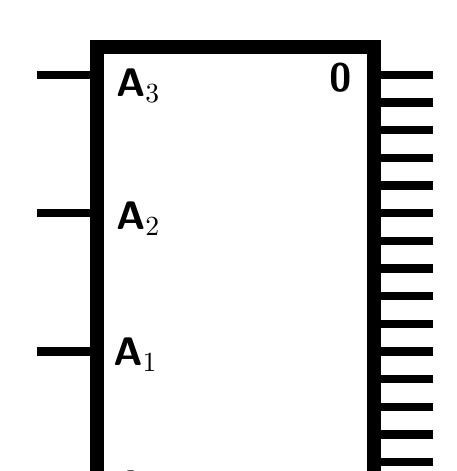
\begin{tikzpicture}[x=1pt,y=-1pt,line cap=rect]
\useasboundingbox (0,0) rectangle (145,150);
\definecolor{custcol_0_0_0}{RGB}{0, 0, 0}
\definecolor{custcol_ff_ff_ff}{RGB}{255, 255, 255}
\draw [line width=3.0pt, custcol_0_0_0 ]  (125.0,47.0) -- (145.0,47.0) ;
\draw [line width=3.0pt, custcol_0_0_0 ]  (125.0,17.0) -- (145.0,17.0) ;
\draw [line width=3.0pt, custcol_0_0_0 ]  (125.0,27.0) -- (145.0,27.0) ;
\draw [line width=3.0pt, custcol_0_0_0 ]  (125.0,37.0) -- (145.0,37.0) ;
\draw [line width=3.0pt, custcol_0_0_0 ]  (125.0,57.0) -- (145.0,57.0) ;
\draw [line width=3.0pt, custcol_0_0_0 ]  (125.0,67.0) -- (145.0,67.0) ;
\draw [line width=3.0pt, custcol_0_0_0 ]  (125.0,77.0) -- (145.0,77.0) ;
\draw [line width=3.0pt, custcol_0_0_0 ]  (125.0,87.0) -- (145.0,87.0) ;
\draw [line width=3.0pt, custcol_0_0_0 ]  (125.0,97.0) -- (145.0,97.0) ;
\draw [line width=3.0pt, custcol_0_0_0 ]  (125.0,107.0) -- (145.0,107.0) ;
\draw [line width=3.0pt, custcol_0_0_0 ]  (125.0,117.0) -- (145.0,117.0) ;
\draw [line width=3.0pt, custcol_0_0_0 ]  (125.0,127.0) -- (145.0,127.0) ;
\draw [line width=3.0pt, custcol_0_0_0 ]  (125.0,137.0) -- (145.0,137.0) ;
\draw [line width=3.0pt, custcol_0_0_0 ]  (125.0,147.0) -- (145.0,147.0) ;
\draw [line width=3.0pt, custcol_0_0_0 ]  (125.0,157.0) -- (145.0,157.0) ;
\draw [line width=3.0pt, custcol_0_0_0 ]  (125.0,167.0) -- (145.0,167.0) ;
\draw [line width=3.0pt, custcol_0_0_0 ]  (5.0,17.0) -- (25.0,17.0) ;
\draw [line width=3.0pt, custcol_0_0_0 ]  (5.0,67.0) -- (25.0,67.0) ;
\draw [line width=3.0pt, custcol_0_0_0 ]  (5.0,117.0) -- (25.0,117.0) ;
\draw [line width=3.0pt, custcol_0_0_0 ]  (5.0,167.0) -- (25.0,167.0) ;
\draw [line width=5.0pt, custcol_0_0_0 ]  (25.0,7.0) -- (124.0,7.0) ;
\draw [line width=5.0pt, custcol_0_0_0 ]  (125.0,7.0) -- (125.0,176.0) ;
\draw [line width=5.0pt, custcol_0_0_0 ]  (125.0,177.0) -- (26.0,177.0) ;
\draw [line width=5.0pt, custcol_0_0_0 ]  (25.0,177.0) -- (25.0,8.0) ;
\fontsize{14pt}{14pt}\fontseries{bx}\sffamily\selectfont\node[inner sep=0, outer sep=0, custcol_0_0_0, anchor=base west] at  (109.0,23.0)  {\textbf{0}};
\fontsize{14pt}{14pt}\fontseries{bx}\sffamily\selectfont\node[inner sep=0, outer sep=0, custcol_0_0_0, anchor=base west] at  (31.0,122.0)  {A$_1$};
\fontsize{14pt}{14pt}\fontseries{bx}\sffamily\selectfont\node[inner sep=0, outer sep=0, custcol_0_0_0, anchor=base west] at  (32.0,170.0)  {A$_0$};
\fontsize{14pt}{14pt}\fontseries{bx}\sffamily\selectfont\node[inner sep=0, outer sep=0, custcol_0_0_0, anchor=base west] at  (32.0,73.0)  {A$_2$};
\fontsize{14pt}{14pt}\fontseries{bx}\sffamily\selectfont\node[inner sep=0, outer sep=0, custcol_0_0_0, anchor=base west] at  (32.0,25.0)  {A$_3$};
\fill [line width=1.0pt, custcol_0_0_0]  (25.0,17.0) ellipse (2.0 and 2.0 );
\fill [line width=1.0pt, custcol_0_0_0]  (25.0,67.0) ellipse (2.0 and 2.0 );
\fill [line width=1.0pt, custcol_0_0_0]  (25.0,117.0) ellipse (2.0 and 2.0 );
\fill [line width=1.0pt, custcol_0_0_0]  (25.0,167.0) ellipse (2.0 and 2.0 );
\fill [line width=1.0pt, custcol_0_0_0]  (125.0,17.0) ellipse (2.0 and 2.0 );
\fill [line width=1.0pt, custcol_0_0_0]  (125.0,27.0) ellipse (2.0 and 2.0 );
\fill [line width=1.0pt, custcol_0_0_0]  (125.0,37.0) ellipse (2.0 and 2.0 );
\fill [line width=1.0pt, custcol_0_0_0]  (125.0,47.0) ellipse (2.0 and 2.0 );
\fill [line width=1.0pt, custcol_0_0_0]  (125.0,57.0) ellipse (2.0 and 2.0 );
\fill [line width=1.0pt, custcol_0_0_0]  (125.0,67.0) ellipse (2.0 and 2.0 );
\fill [line width=1.0pt, custcol_0_0_0]  (125.0,77.0) ellipse (2.0 and 2.0 );
\fill [line width=1.0pt, custcol_0_0_0]  (125.0,87.0) ellipse (2.0 and 2.0 );
\fill [line width=1.0pt, custcol_0_0_0]  (125.0,97.0) ellipse (2.0 and 2.0 );
\fill [line width=1.0pt, custcol_0_0_0]  (125.0,107.0) ellipse (2.0 and 2.0 );
\fill [line width=1.0pt, custcol_0_0_0]  (125.0,117.0) ellipse (2.0 and 2.0 );
\fill [line width=1.0pt, custcol_0_0_0]  (125.0,127.0) ellipse (2.0 and 2.0 );
\fill [line width=1.0pt, custcol_0_0_0]  (125.0,137.0) ellipse (2.0 and 2.0 );
\fill [line width=1.0pt, custcol_0_0_0]  (125.0,147.0) ellipse (2.0 and 2.0 );
\fill [line width=1.0pt, custcol_0_0_0]  (125.0,157.0) ellipse (2.0 and 2.0 );
\fill [line width=1.0pt, custcol_0_0_0]  (125.0,167.0) ellipse (2.0 and 2.0 );
\end{tikzpicture}
}